% \documentclass{standalone} 
% standalone mode causes trouble when using tikz
% http://www.texample.net/tikz/examples/system-combination/

\documentclass[class=article,border=2pt]{standalone}
\usepackage{tikz}
\usetikzlibrary{arrows,shapes,positioning,shadows,trees}

\tikzset{
  basic/.style  = {draw, text width=3cm, drop shadow, font=\sffamily, rectangle},
  root/.style   = {basic, rounded corners=2pt, thin, align=center, fill=green!30},
  crawler/.style = {basic, rounded corners=2pt, thin, align=center, fill=green!30},
  level 2/.style = {basic, rounded corners=6pt, thin,align=center, fill=green!60, text width=8em},
  level 3/.style = {basic, thin, align=left, fill=pink!60},
  level 4/.style = {basic, thin, align=left, fill=pink!60, text width=6.5em}
}

\begin{document}
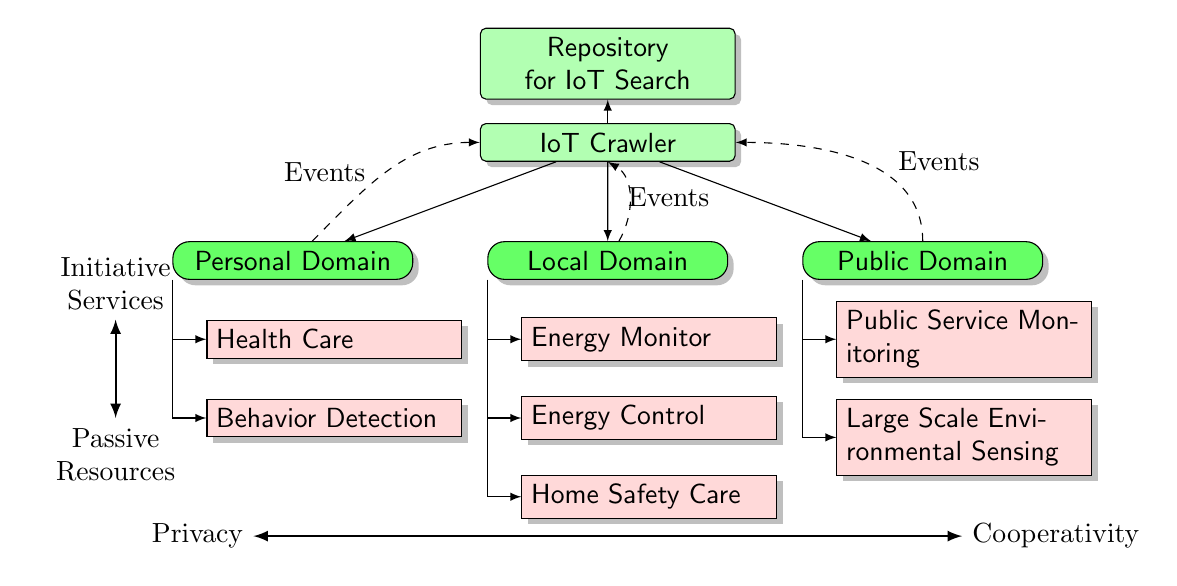
\begin{tikzpicture}[
  level 1/.style={sibling distance=40mm},
  edge from parent/.style={->,draw},
  >=latex]

% root of the the initial tree, level 1
\node [root](r) {Repository\\ for IoT Search};

% The first level, as children of the initial tree
\node [crawler][below of = r](cw) {IoT Crawler}
  child {node[level 2] (c1) {    Personal Domain    }}
  child {node[level 2] (c2) {    Local Domain     }}
  child {node[level 2] (c3) {    Public Domain   }};

\draw [<-] (r)--(cw);
\draw (c1) edge[out=45, in=180,->,dashed] node[xshift=-0.8cm]{Events} (cw.west);
\draw (c2) edge[out=60, in=330,->,dashed] node[xshift=0.5cm]{Events} (cw.south);
\draw (c3) edge[out=90, in=0,->,dashed] node[xshift=1cm]{Events} (cw.east);

% The second level, relatively positioned nodes
\begin{scope}[every node/.style={level 3}]
\node [below of = c1, xshift=15pt] (c11) {Health Care};
\node [below of = c11] (c12) {Behavior Detection};

\node [below of = c2, xshift=15pt] (c21) {Energy Monitor};
\node [below of = c21] (c22) {Energy Control};
\node [below of = c22] (c23) {Home Safety Care};

\node [below of = c3, xshift=15pt] (c31) {Public Service Monitoring};
\node [below of = c31, yshift=-7pt] (c32) {Large Scale Environmental Sensing};
\end{scope}

% lines from each level 1 node to every one of its "children"
\foreach \value in {1,2}
  \draw[->] (c1.south west) |- (c1\value.west);
\foreach \value in {1,2,3}
  \draw[->] (c2.south west) |- (c2\value.west);
\foreach \value in {1,2}
  \draw[->] (c3.south west) |- (c3\value.west);

% axis
\draw[thick,<->] (-4.5,-6.0) node[anchor=east]{Privacy} -- (4.5,-6.0) node[anchor=west]{Cooperativity};
\draw[thick,<->] (-6.25,-3.25) node[anchor=south, text width=2cm, align=center]{Initiative\\ Services} -- 
				(-6.25,-4.5) node[anchor=north, text width=2cm, align=center]{Passive\\ Resources};
% \draw[thick,->] (0,0) -- (0,4.5) node[anchor=south east] {y axis};

    
\end{tikzpicture}
\end{document}